\section[REBOUND]{REBOUND:\ Código N-cuerpos multipropósito de código abierto para dinámica colisional}

REBOUND (Rein \& Liu, 2012)~\cite{Rein2012} se define como un código numérico de N-cuerpos, multipropósito y de código abierto, distribuido bajo la licencia GPLv3~\cite{Rein2012}. Fue diseñado primordialmente para abordar problemas de dinámica colisional, como los encontrados en anillos planetarios, pero es igualmente capaz de resolver el problema clásico de N-cuerpos en sistemas puramente gravitacionales~\cite{Rein2012} [Abstract, Sec. 1]. Su desarrollo buscó llenar un vacío existente en cuanto a códigos públicos disponibles para la simulación de dinámica colisional compleja~\cite{Rein2012} [Sec. 1].

\subsection{Principios Fundamentales y Funcionamiento}

La filosofía central de REBOUND es su alta modularidad~\cite{Rein2012} [Abstract, Sec. 2.2]. Está escrito enteramente en C (conforme al estándar ISO C99) y diseñado para compilar y ejecutarse en plataformas modernas compatibles con POSIX (como Linux, Unix y Mac OSX)~\cite{Rein2012} [Sec. 2, Sec. 2.1]. La estructura modular permite al usuario seleccionar y combinar diferentes componentes mediante el uso de enlaces simbólicos, sin necesidad de modificar el código fuente principal. Esto facilita la adaptación del código a una amplia variedad de problemas astrofísicos y de otras disciplinas~\cite{Rein2012} [Sec. 2.2]. Los módulos intercambiables incluyen:

\begin{enumerate}
    \item \textbf{Integradores Numéricos:} REBOUND implementa varios integradores, mayormente basados en el esquema simpléctico de segundo orden Drift-Kick-Drift (DKD). Es importante notar que la naturaleza simpléctica se pierde formalmente si se introducen aproximaciones en el cálculo de la gravedad, colisiones o fuerzas dependientes de la velocidad~\cite{Rein2012} [Sec. 3]. Los integradores principales son:
    \begin{itemize}
        \item \textbf{Leap-frog:} Un integrador simpléctico estándar de segundo orden para marcos no rotacionales~\cite{Rein2012} [Sec. 3.1].
        \item \textbf{Wisdom-Holman (WH):} Un mapeo simpléctico de variables mixtas que integra el movimiento kepleriano de forma exacta durante el paso de deriva (\textit{drift}). Es muy preciso para problemas dominados por un potencial central $1/r$, pero computacionalmente más costoso que Leap-frog debido a la resolución iterativa de la ecuación de Kepler~\cite{Rein2012} [Sec. 3.2].
        \item \textbf{Symplectic Epicycle Integrator (SEI):} Diseñado para la aproximación de Hill (utilizada en láminas de cizallamiento o \textit{shearing sheets}), opera en un marco rotacional y es computacionalmente rápido~\cite{Rein2012} [Sec. 3.3].
    \end{itemize}
    REBOUND utiliza un paso de tiempo (\textit{timestep}) fijo para todas las partículas por defecto, lo cual es crucial para mantener las propiedades simplécticas de los integradores correspondientes. Es responsabilidad del usuario asegurar que el paso de tiempo sea suficientemente pequeño para la convergencia numérica~\cite{Rein2012} [Sec. 3].

    \item \textbf{Cálculo de Gravedad:} Se proporcionan dos módulos principales para calcular las fuerzas gravitacionales~\cite{Rein2012} [Sec. 4]:
    \begin{itemize}
        \item \textbf{Suma Directa:} Calcula la interacción entre todos los pares de partículas activas ($N_{\text{active}}$) de forma exacta (ecuación 1 en~\cite{Rein2012}). Su costo computacional escala como $O(N \cdot N_{\text{active}})$, siendo eficiente solo para un número bajo de partículas masivas ($N_{\text{active}} \le 10^2$)~\cite{Rein2012} [Sec. 4.1]. Permite incluir un parámetro de suavizado gravitacional ($b$) para evitar aceleraciones extremas en encuentros cercanos~\cite{Rein2012} [Eq. 1].
        \item \textbf{Octree (Árbol Octal):} Implementa el algoritmo de Barnes \& Hut (1986) para aproximar las fuerzas de largo alcance, reduciendo la complejidad computacional a $O(N \log N)$~\cite{Rein2012} [Sec. 4.2]. Agrupa jerárquicamente las partículas distantes y utiliza su centro de masa (y opcionalmente su tensor cuadrupolar, siguiendo a Hernquist, 1987) para calcular la fuerza, basándose en un criterio de ángulo de apertura ($\theta_{\text{crit}}$). Este módulo está completamente paralelizado usando MPI (con descomposición estática de dominio y árboles esenciales distribuidos) y OpenMP~\cite{Rein2012} [Sec. 4.2, Sec. 7].
        % Sugerencia Visual:
        % [Aquí podría insertarse una figura adaptada de la Fig. 4 de~\cite{Rein2012} para ilustrar la convergencia
        % de la precisión de la fuerza en función de theta_crit y la mejora al incluir el término cuadrupolar].
    \end{itemize}

    \item \textbf{Detección de Colisiones:} REBOUND incluye varios módulos para detectar colisiones, modeladas como interacciones entre esferas duras con un coeficiente de restitución $\epsilon$ especificado por el usuario~\cite{Rein2012} [Sec. 5]. Las colisiones detectadas en un paso de tiempo se resuelven en orden aleatorio para evitar sesgos~\cite{Rein2012} [Sec. 5]. Los métodos son:
    \begin{itemize}
        \item \textbf{Búsqueda Directa del Vecino Más Cercano:} Comprueba el solapamiento de todas las parejas de partículas al final del paso de tiempo. Escala como $O(N^2)$~\cite{Rein2012} [Sec. 5.1].
        \item \textbf{Octree:} Utiliza la estructura del árbol octal para buscar vecinos cercanos y detectar solapamientos, con una complejidad promedio de $O(N \log N)$. Puede usar la misma estructura del árbol de gravedad y está paralelizado (MPI/OpenMP)~\cite{Rein2012} [Sec. 5.2].
        \item \textbf{Algoritmo de Barrido Plano (Plane-Sweep):} Dos variantes (cartesiana en $x$ y angular en $\phi$) basadas en el algoritmo de Bentley \& Ottmann (1979), pero simplificadas. Aproxima las trayectorias de las partículas como líneas rectas durante un paso de tiempo. Mueve un plano conceptual a través del dominio, manteniendo una lista de partículas activas intersectadas por el plano y comprobando colisiones solo dentro de esa lista. Su complejidad es $O(N \cdot N_{\text{SWEEPL}})$, donde $N_{\text{SWEEPL}}$ es el número promedio de partículas en la lista activa. Es significativamente más eficiente que los métodos basados en árboles para simulaciones cuasi-bidimensionales o muy elongadas (donde $N_{\text{SWEEPL}}$ es pequeño), como anillos planetarios densos o simulaciones en láminas de cizallamiento~\cite{Rein2012} [Sec. 5.3].
        \begin{figure}[H]
            \centering
            % Descomenta la siguiente línea e inserta la ruta a tu imagen
            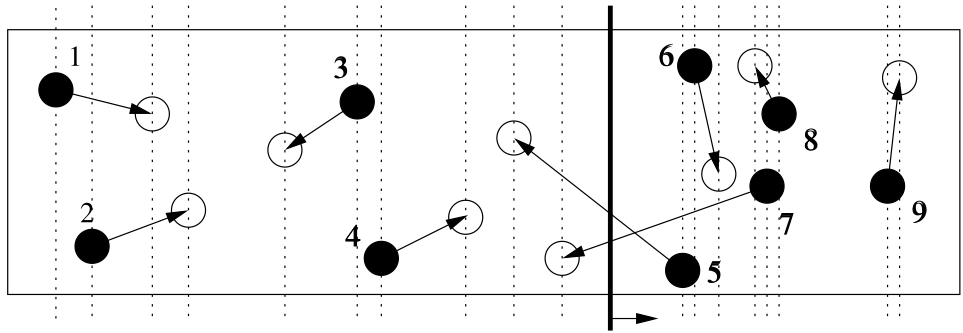
\includegraphics[width=\textwidth]{img/marcoTeorico/Algoritmo_de_barrido_plano.png}
            %\fbox{\parbox{0.8\textwidth}{\centering Placeholder: Figura Esquema de la Jerarquía de Celdas y Listas de Interacción}}
            \caption{Ilustración del algoritmo de barrido plano. El plano interseca las trayectorias de las partículas 5 y 7. Véanse los detalles en el texto adaptado de~\cite{Rein2012}.}%
            \label{fig:plane_sweep_algorithm}
        \end{figure}
    \end{itemize}

    \item \textbf{Condiciones de Contorno:} Soporta condiciones de contorno abiertas (las partículas que salen son eliminadas), periódicas (implementadas con cajas fantasma) y de lámina de cizallamiento (\textit{shear-periodic})~\cite{Rein2012} [Sec. 2.3].
\end{enumerate}

\subsection{Contexto Histórico y Origen}

El código fue presentado por H. Rein y S.-F. Liu en 2012~\cite{Rein2012}, aunque versiones precursoras ya se habían utilizado en publicaciones anteriores (e.g., Rein \& Papaloizou, 2010; Crida et al., 2010; Rein et al., 2010)~\cite{Rein2012} [Sec. 1]. Nació de la necesidad de contar con una herramienta pública, flexible y eficiente para estudiar la dinámica de sistemas astrofísicos donde las colisiones juegan un papel crucial, como los anillos de Saturno o los discos protoplanetarios~\cite{Rein2012} [Sec. 1].

\subsection{Variantes y Enfoques Principales}

Más que variantes distintas del código, REBOUND ofrece diferentes enfoques de simulación a través de la combinación de sus módulos. El usuario puede configurar la simulación eligiendo el integrador más adecuado (e.g., WH para alta precisión a largo plazo en sistemas planetarios, SEI para láminas de cizallamiento, Leap-frog como opción general), el método de cálculo de gravedad (directo para pocos cuerpos, árbol para muchos) y el algoritmo de detección de colisiones (directo, árbol, o barrido plano según la geometría y densidad del problema)~\cite{Rein2012} [Sec. 2.2, Sec. 3, Sec. 4, Sec. 5].

\subsection{Aplicaciones Típicas}

La literatura documenta el uso de REBOUND en una variedad de problemas astrofísicos:
\begin{itemize}
    \item Simulación de anillos planetarios, incluyendo el estudio de su viscosidad y estructuras inducidas por satélites~\cite{Rein2012} [Sec. 1, Sec. 6.4].
    \item Formación de planetesimales a partir de enjambres de partículas en discos protoplanetarios~\cite{Rein2012} [Sec. 1].
    \item Estudio de discos de transición y de escombros (utilizando superpartículas)~\cite{Rein2012} [Sec. 1].
    \item Problemas clásicos de N-cuerpos, como la integración a largo plazo de la dinámica del Sistema Solar~\cite{Rein2012} [Sec. 1, Sec. 6.3].
\end{itemize}
Aunque diseñado para astrofísica, su estructura modular lo hace potencialmente aplicable a otros campos que involucren dinámica de partículas, como la dinámica molecular o flujos granulares~\cite{Rein2012} [Abstract].

\subsection{Ventajas y Limitaciones}

Las principales \textbf{ventajas} de REBOUND, según se desprenden de~\cite{Rein2012}, son:
\begin{itemize}
    \item \textbf{Código Abierto y Gratuito:} Accesible para la comunidad científica bajo licencia GPLv3~\cite{Rein2012} [Sec. 1].
    \item \textbf{Modularidad y Flexibilidad:} Altamente personalizable para diferentes problemas~\cite{Rein2012} [Abstract, Sec. 2.2].
    \item \textbf{Eficiencia y Escalabilidad:} Demuestra buen escalado en paralelo (tanto fuerte como débil) usando MPI y OpenMP, permitiendo simulaciones con un gran número de partículas en clústeres de cómputo~\cite{Rein2012} [Abstract, Sec. 7].
    \item \textbf{Variedad de Métodos:} Ofrece múltiples opciones de integradores, cálculo de gravedad y detección de colisiones~\cite{Rein2012} [Sec. 3, Sec. 4, Sec. 5].
    \item \textbf{Precisión:} Los integradores simplécticos son adecuados para integraciones a largo plazo, y se conserva la energía y el momento hasta la precisión de la máquina en colisiones elásticas~\cite{Rein2012} [Sec. 3, Sec. 6.2].
\end{itemize}

Las \textbf{limitaciones} inherentes o aspectos a considerar son:
\begin{itemize}
    \item \textbf{Paso de Tiempo Fijo:} Generalmente requerido por los integradores simplécticos, lo que puede ser ineficiente si ocurren escalas de tiempo muy diferentes en el sistema~\cite{Rein2012} [Sec. 3]. El usuario debe elegirlo cuidadosamente.
    \item \textbf{Pérdida de Simplecticidad:} Las propiedades simplécticas se pierden si se usan aproximaciones (árbol de gravedad), colisiones o fuerzas no conservativas~\cite{Rein2012} [Sec. 3].
    \item \textbf{Aproximaciones:} Los métodos de árbol para gravedad y colisiones son aproximados, con una precisión que depende de parámetros como $\theta_{\text{crit}}$~\cite{Rein2012} [Sec. 4.2, Sec. 6.1]. El método de barrido plano aproxima las trayectorias como líneas rectas entre pasos~\cite{Rein2012} [Sec. 5.3, Fig. 2].
    \item \textbf{Rendimiento:} El rendimiento del árbol puede degradarse si el número de partículas por nodo MPI es muy bajo debido al costo de comunicación~\cite{Rein2012} [Sec. 7.1]. La eficiencia del barrido plano depende crucialmente de la dimensionalidad efectiva del problema~\cite{Rein2012} [Sec. 5.3, Sec. 9].
\end{itemize}
